% --------------------------------------------------------------------------- %
% Poster for the ECCS 2011 Conference about Elementary Dynamic Networks.      %
% --------------------------------------------------------------------------- %
% Created with Brian Amberg's LaTeX Poster Template. Please refer for the     %
% attached README.md file for the details how to compile with `pdflatex`.     %
% --------------------------------------------------------------------------- %
% $LastChangedDate:: 2011-09-11 10:57:12 +0200 (V, 11 szept. 2011)          $ %
% $LastChangedRevision:: 128                                                $ %
% $LastChangedBy:: rlegendi                                                 $ %
% $Id:: poster.tex 128 2011-09-11 08:57:12Z rlegendi                        $ %
% --------------------------------------------------------------------------- %
\documentclass[a0paper,portrait]{baposter}

\usepackage{relsize}		% For \smaller
\usepackage{url}			% For \url
% \usepackage{epstopdf}	% Included EPS files automatically converted to PDF to include with pdflatex

%%% Global Settings %%%%%%%%%%%%%%%%%%%%%%%%%%%%%%%%%%%%%%%%%%%%%%%%%%%%%%%%%%%

\graphicspath{{pix/}}	% Root directory of the pictures 
% \tracingstats=2			% Enabled LaTeX logging with conditionals

%%% Color Definitions %%%%%%%%%%%%%%%%%%%%%%%%%%%%%%%%%%%%%%%%%%%%%%%%%%%%%%%%%

\definecolor{bordercol}{RGB}{149, 149, 149 }
\definecolor{headercol1}{RGB}{199,230,251}
\definecolor{headercol2}{RGB}{199,230,251}
\definecolor{headerfontcol}{RGB}{0, 0, 0}
\definecolor{boxcolor}{RGB}{255, 255, 255}

%%%%%%%%%%%%%%%%%%%%%%%%%%%%%%%%%%%%%%%%%%%%%%%%%%%%%%%%%%%%%%%%%%%%%%%%%%%%%%%%
%%% Utility functions %%%%%%%%%%%%%%%%%%%%%%%%%%%%%%%%%%%%%%%%%%%%%%%%%%%%%%%%%%

%%% Save space in lists. Use this after the opening of the list %%%%%%%%%%%%%%%%
\newcommand{\compresslist}{
	\setlength{\itemsep}{1pt}
	\setlength{\parskip}{0pt}
	\setlength{\parsep}{0pt}
}

%%%%%%%%%%%%%%%%%%%%%%%%%%%%%%%%%%%%%%%%%%%%%%%%%%%%%%%%%%%%%%%%%%%%%%%%%%%%%%%
%%% Document Start %%%%%%%%%%%%%%%%%%%%%%%%%%%%%%%%%%%%%%%%%%%%%%%%%%%%%%%%%%%%
%%%%%%%%%%%%%%%%%%%%%%%%%%%%%%%%%%%%%%%%%%%%%%%%%%%%%%%%%%%%%%%%%%%%%%%%%%%%%%%

\begin{document}
\typeout{Poster rendering started}

%%% Setting Background Image %%%%%%%%%%%%%%%%%%%%%%%%%%%%%%%%%%%%%%%%%%%%%%%%%%
\background{
	\begin{tikzpicture}[remember picture,overlay]%
	\draw (current page.north west)+(-2em,2em) node[anchor=north west]
	{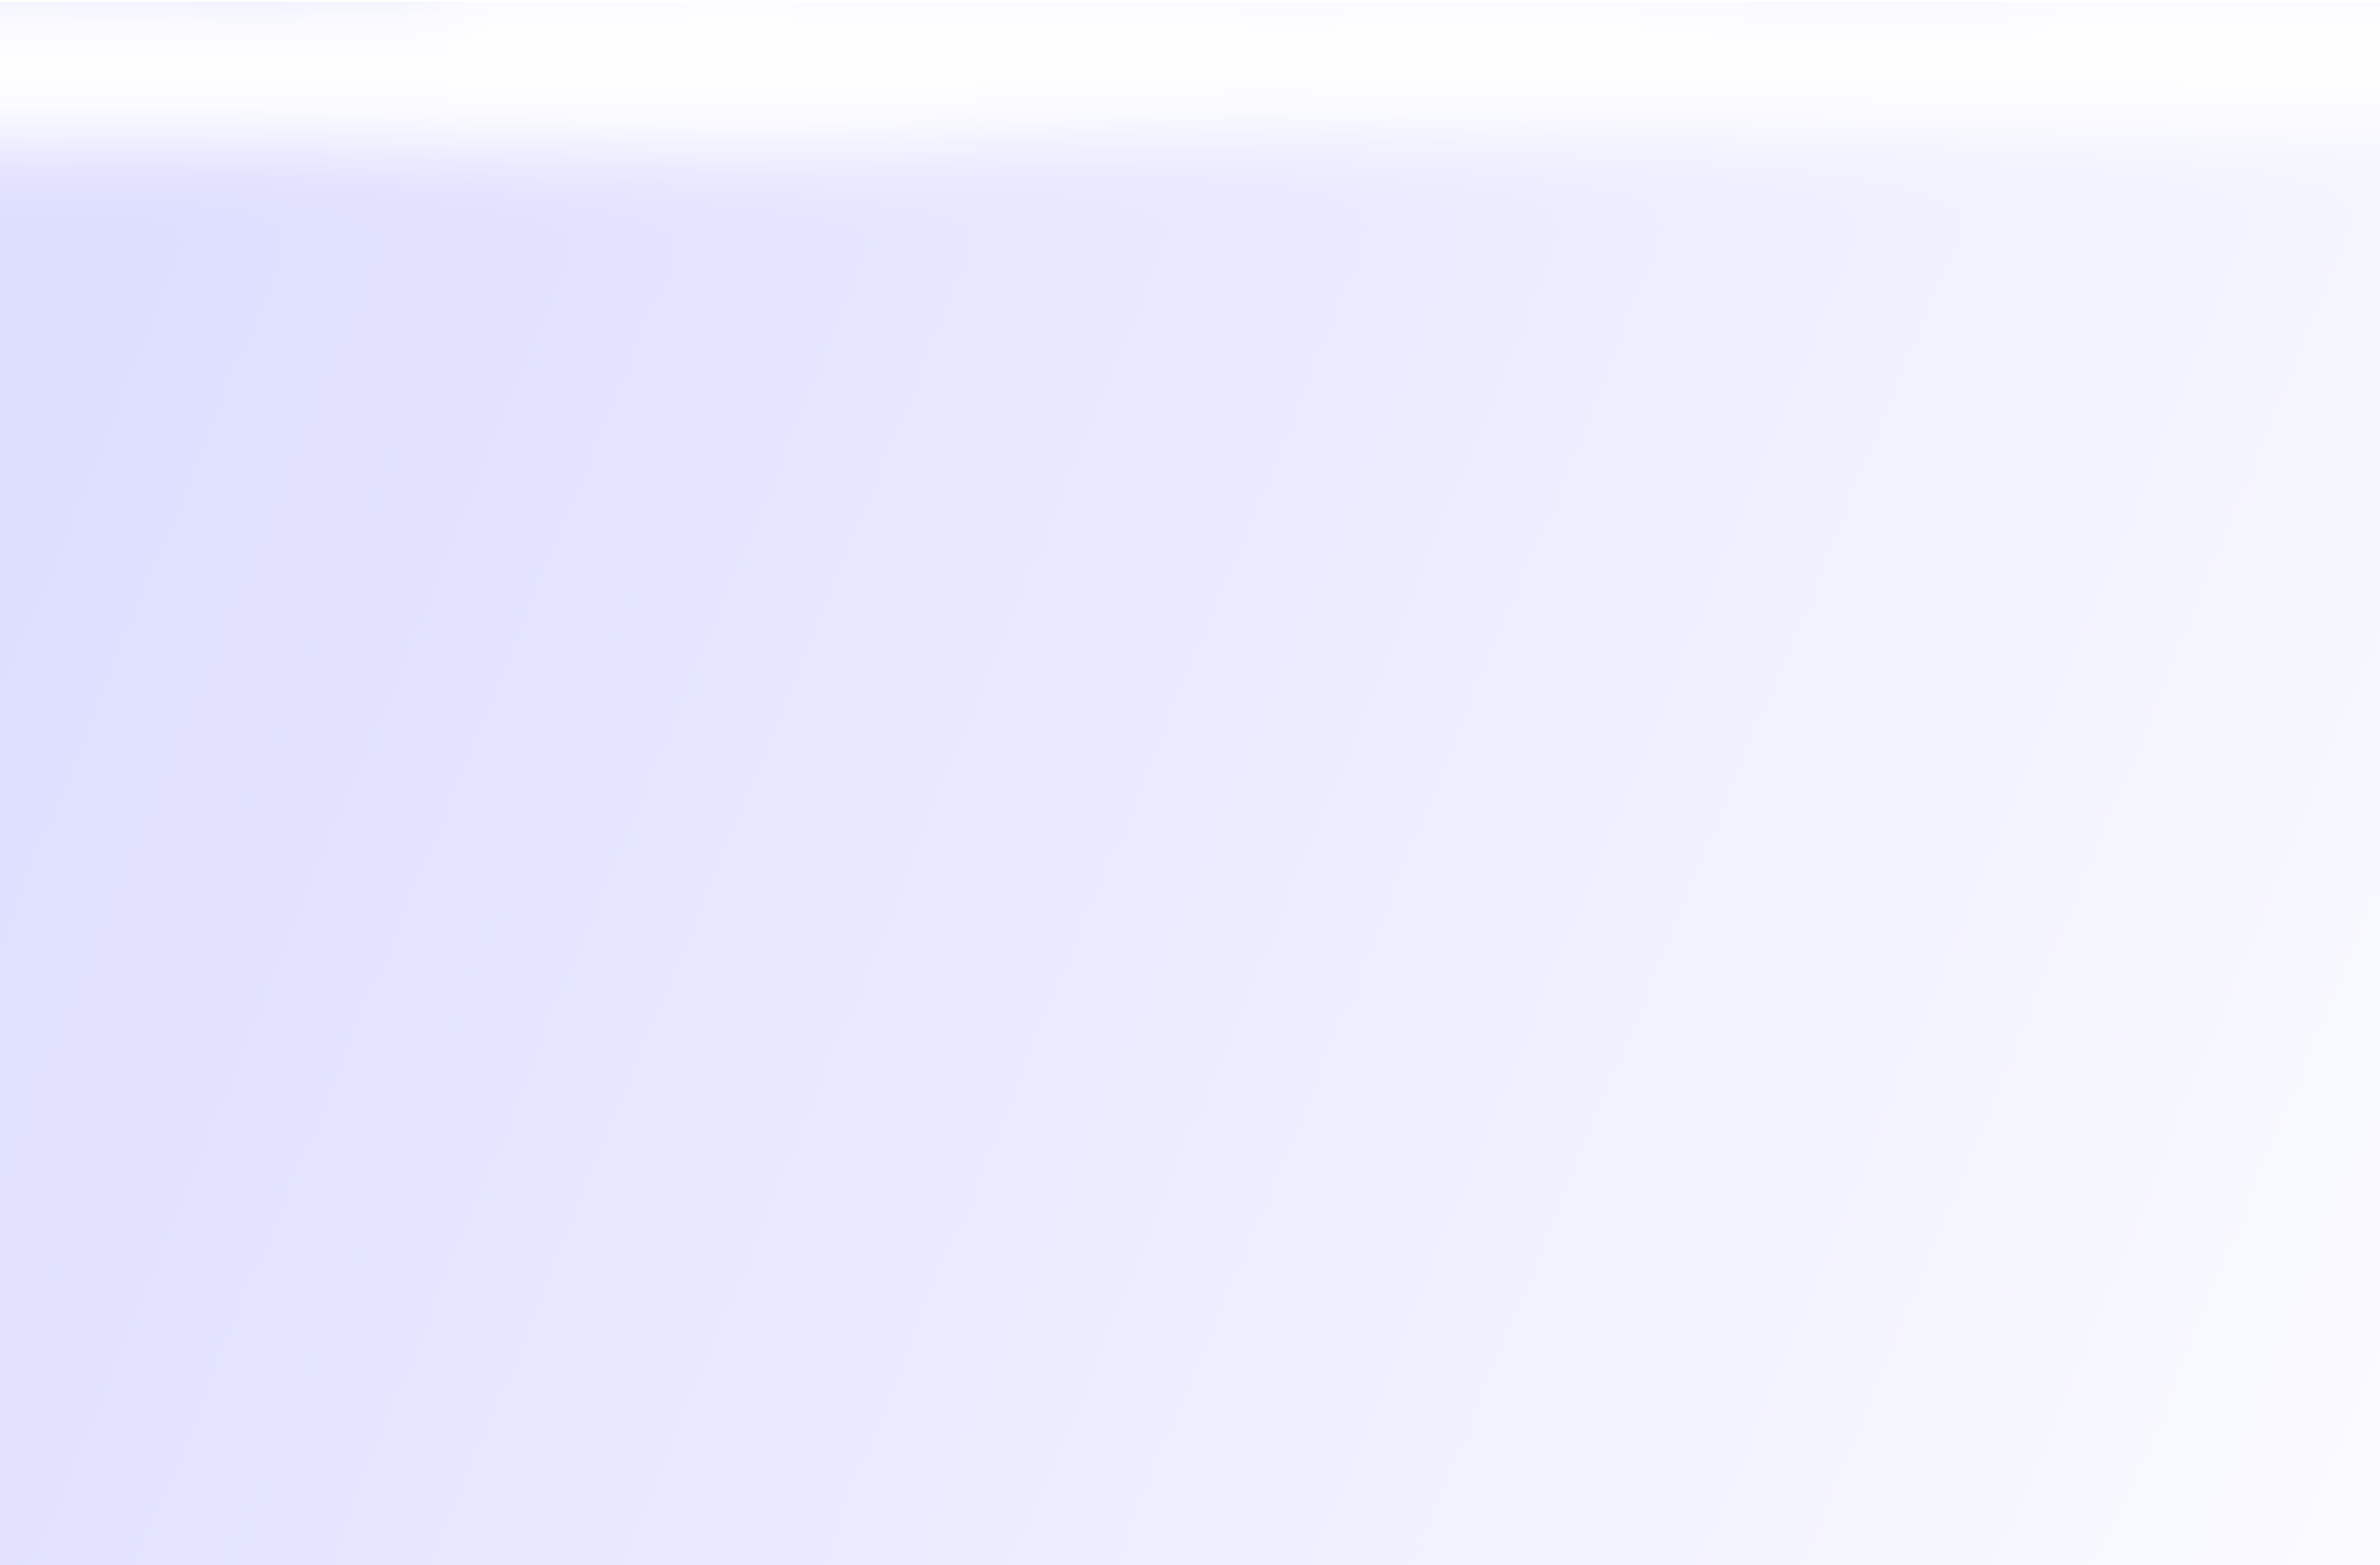
\includegraphics[height=1.1\textheight]{background}};
	\end{tikzpicture}
}

%%% General Poster Settings %%%%%%%%%%%%%%%%%%%%%%%%%%%%%%%%%%%%%%%%%%%%%%%%%%%
%%%%%% Eye Catcher, Title, Authors and University Images %%%%%%%%%%%%%%%%%%%%%%
\begin{poster}{
	grid=false,
    columns=3,
    columnWidths={0.2, 0.2,0.6},
	borderColor=bordercol,
	headerColorOne=headercol1,
	headerColorTwo=headercol2,
	headerFontColor=headerfontcol,
	% Only simple background color used, no shading, so boxColorTwo isn't necessary
	boxColorOne=boxcolor,
	headershape=roundedright,
	headerfont=\Large\sf\bf,
	textborder=rectangle,
	background=user,
	headerborder=open,
  boxshade=plain
}
%%% Eye Cacther %%%%%%%%%%%%%%%%%%%%%%%%%%%%%%%%%%%%%%%%%%%%%%%%%%%%%%%%%%%%%%%
{
	Eye Catcher, empty if option eyecatcher=false - unused
}
%%% Title %%%%%%%%%%%%%%%%%%%%%%%%%%%%%%%%%%%%%%%%%%%%%%%%%%%%%%%%%%%%%%%%%%%%%
{\sf\bf
	Fluorescencia Resonante Intermitente y Trayectorias de Saltos Cuánticos
}
%%% Authors %%%%%%%%%%%%%%%%%%%%%%%%%%%%%%%%%%%%%%%%%%%%%%%%%%%%%%%%%%%%%%%%%%%
{
	\vspace{1em} Kevin Mart\'inez Franco,\\
	{\smaller kevin.martinez@uaem.edu.mx, }
}
%%% Logo %%%%%%%%%%%%%%%%%%%%%%%%%%%%%%%%%%%%%%%%%%%%%%%%%%%%%%%%%%%%%%%%%%%%%%
{
% The logos are compressed a bit into a simple box to make them smaller on the result
% (Wasn't able to find any bigger of them.)
\setlength\fboxsep{0pt}
\setlength\fboxrule{0.2pt}
	\fbox{
	\begin{minipage}[t]{0.15\textwidth}
            
\includegraphics[width=7em,height=6em]{logos/uaem.png}
        \end{minipage}%
        \hfill
        \begin{minipage}[t]{0.15\textwidth}
            \flushright
            
\includegraphics[width=10em,height=4.5em]{logos/ciicap.png}
        \end{minipage}
	}
}


\headerbox{Planteamiento del problema}{name=problem,column=0,row=0}
{
Abordamos el fenómeno de fluorescencia resonante intermitente, que describe la alternancia aleatoria entre per\'iodos de emisión frecuente de fotones ("brillantes") y periodos de nula emisión ("oscuros") en un átomo excitado por un láser \cite{PlKn}. 

Consideramos un átomo de tres niveles interactuando con un láser que excita la transici\'on 
$|e \rangle - |g \rangle$ con frecuencia de Rabi $\Omega$, y que decae a raz\'on $\gamma$, generando un per\'iodo brillante. 
El estado $|e \rangle$ decae ocasionalmente a raz\'on $\gamma_d$ a un estado metaestable $|a \rangle$ que interrumpe la fluorescencia en $|e \rangle - |g \rangle$. Al decaer el estado $|a \rangle$ a $|g \rangle$ a raz\'on $\gamma_a$ vuelve la fluorescencia. Las razones de emisi\'on espont\'anea cumplen 
$\gamma \gg \gamma_d,\gamma_a$.

Para simular este proceso, utilizamos el método de Trayectorias Cuánticas \cite{Carmichael}, que modela la dinámica de emisión fotónica del sistema. 
\begin{center}
   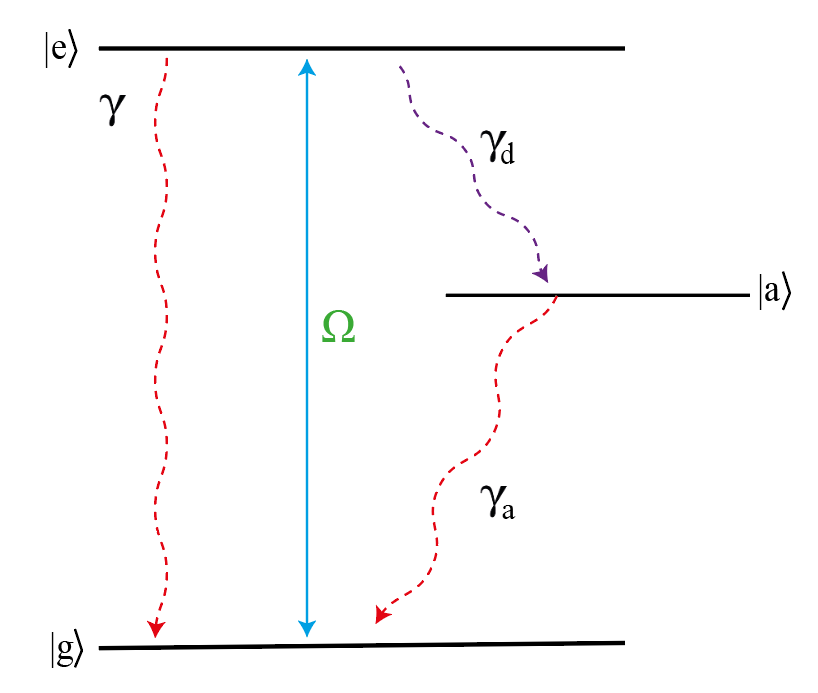
\includegraphics[width=0.8\linewidth]{1 sistema.png} 
\end{center}
}

\headerbox{Trayectorias Cu\'anticas}{name=models,span=1,column=0,below=problem}{
Para simular una trayectoria cu\'antica de saltos resolvemos la ecuaci\'on de Schr\"odinger $i\hbar \dot{|\Psi \rangle} =H_{\mathrm{eff}} |\Psi \rangle$, donde $H_{\mathrm{eff}} = H - i \frac{\gamma}{2} A_{ee} -i \frac{\gamma_d}{2} A_{ee} - i \frac{\gamma_a}{2} A_{aa}$ es un Hamiltoniano efectivo no-Hermitiano, $H = \Delta A_{eg} A_{ge} + \frac{\Omega}{2} (A_{eg} + A_{ge})$ es el Hamiltoniano de la interacci\'on \'atomo-l\'aser, y los siguientes t\'erminos denotan emisi\'on espont\'anea. 

Una trayectoria consiste en intervalos de evoluci\'on no unitaria hasta que se emite un fot\'on en alguna de las transiciones con 
probabilidad $p_k(t) = \delta t \langle \Psi_c(t) | \mathcal{C}_k^\dagger \mathcal{C}_k | \Psi_c(t) \rangle$, 
donde $\mathcal{C}_k = \sqrt{\gamma_k} A_{kk}$ son los operadores de colapso que representan los diferentes canales de emisión. De no emitirse un fot\'on el sistema contin\'ua siguiendo la ecuaci\'on de Schr\"odinger

El promedio en el ensamble de muchas trayectorias reproduce la evolución del operador de densidad $\rho$, que obedece la ecuación maestra $\dot{\rho} = -\frac{i}{\hbar} [H, \rho] + \mathcal{L}_D \rho$, donde $\mathcal{L}_D$ es el superoperador de Lindblad, que modela las emisiones espontáneas entre los diferentes niveles atómicos. 
}

\headerbox{Referencias}{name=references,column=0,below=models}{
\smaller													% Make the whole text smaller
\vspace{-0.4em} 										% Save some space at the beginning
\bibliographystyle{plain}							% Use plain style
\renewcommand{\section}[2]{\vskip 0.05em}		% Omit "References" title
\begin{thebibliography}{1}							% Simple bibliography with widest label of 1
\itemsep=-0.01em										% Save space between the separation
\setlength{\baselineskip}{0.4em}					% Save space with longer lines

\bibitem{PlKn} M. B. Plenio and P. L. Knight, Rev. Mod. Phys. \textbf{70} 101 (1998). 
%
\bibitem{Carmichael} H. Carmichael, An Open Systems Approach to Quantum Optics (Springer, Berlin, 2002). %
%
\bibitem{Tamm} V. B\"uhner and C. Tamm, Phys. Rev. A \textbf{61} 061801 (2000). 
%
\bibitem{RSHC18} R. Rom\'an-Ancheyta, O. de los Santos-S\'anchez, L. Horvath, and H. M. Castro-Beltr\'an, Phys. Rev. A \textbf{98} 013820 (2018). 

\end{thebibliography}
}




\headerbox{Resultados}{name=density,column=1,span=2,row=0}{
En la Fig.~2, a la izquierda, mostramos un fragmento de una trayectoria t\'ipica, mostrando per\'iodos brillantes con oscilaciones de Rabi, y per\'iodos oscuros. A la derecha mostramos el promedio en un ensamble de 4000 trayectorias, el cual se compara muy bien con el resultado obtenido con la ecuaci\'on maestra. Par\'ametros: $\Omega=3.5\gamma$, $\Delta=0$, $\gamma_d=0.95\gamma$, $\gamma_d=0.05\gamma$, $\gamma_a =0.015 \gamma$. 

\begin{center}
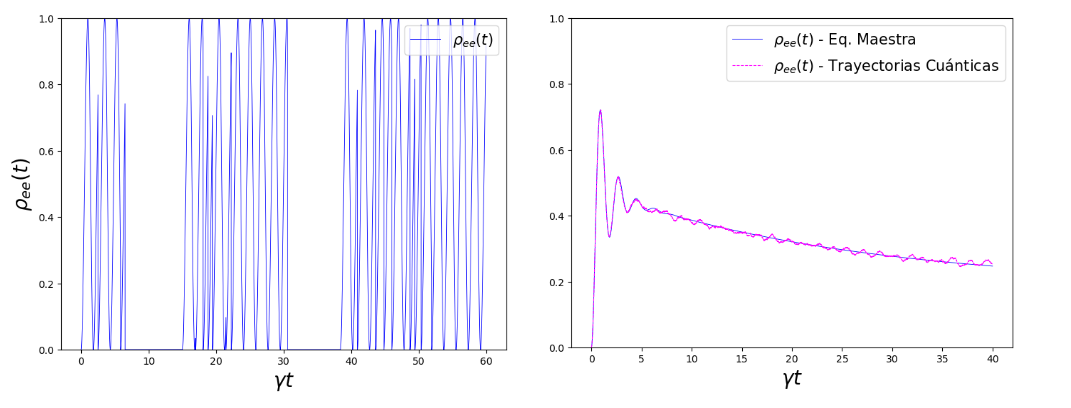
\includegraphics[width=0.8\linewidth]{zoom y meq vs tj.png} 
\end{center}

\\
En un per\'iodo brillante la raz\'on de emisi\'on de fotones es $\gamma \langle \rho_{ee} (t) \rangle$. Un per\'iodo oscuro finaliza cuando se vuelve a emitir un fot\'on en la transici\'on fuerte, iniciando otro per\'iodo brillante. Estos per\'iodos ocurren estoc\'asticamente. 

}


\headerbox{Distribución de Per\'iodos Oscuros y Espectro}
{name=degreeDistribution,column=1,span=2,below=density,above=bottom}{
El procedimiento de c\'alculo de trayectorias permite recoger la informaci\'on de fotoemisiones y estad\'istica de los per\'iodos brillantes y oscuros. Esto se logra mejor si hacemos una trayectoria muy larga en lugar de muchas trayectorias cortas. Se pueden obtener las distribuciones de las duraciones de los periodos oscuros y brillantes, que siguen distribuciones exponenciales: 
$$ P_O = \frac{1}{T_O} e^{-t/T_O}, \qquad  
    P_B = \frac{1}{T_B} e^{-t/T_B} ,$$
con duraciones promedio
$$ T_O = \gamma_a^{-1}, \qquad T_B = \frac{2\Omega^2 + \gamma^2 + 4\Delta^2}{\gamma_d \Omega^2} .$$
La figura 3 muestra las duraciones de los per\'iodos oscuros y su distribuci\'on obtenidas de una trayectoria larga de duraci\'on $\gamma t = 10^6$. 

\vspace{-0.2em}
\begin{center}
	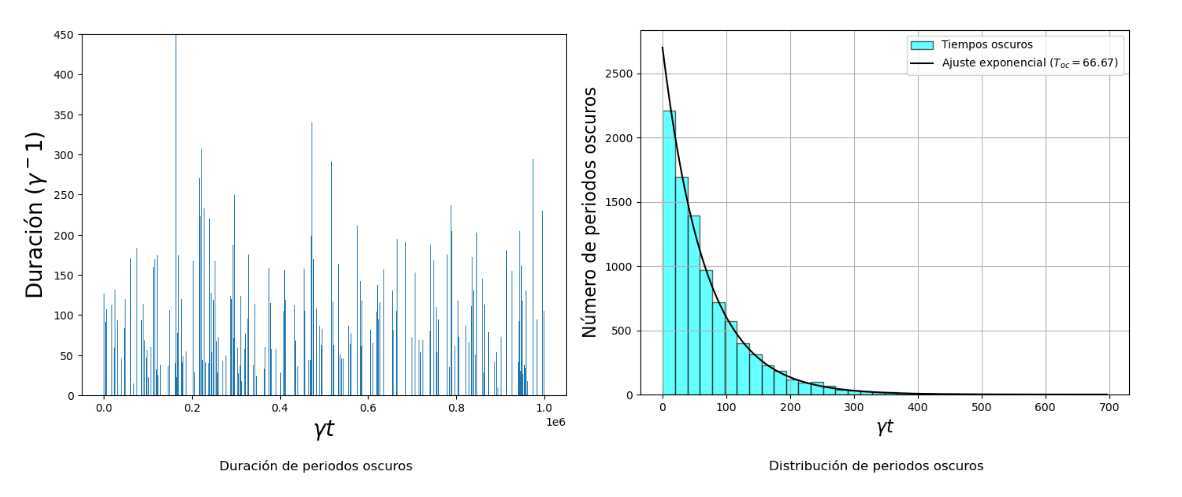
\includegraphics[width=0.8\linewidth]{5 dist dur.png}
\end{center}
\vspace{-0.2em}
Una extensión natural del método de trayectorias de saltos es el uso de \textbf{trayectorias cuánticas difusivas}, que permiten simular la medición del espectro mediante detección heterodina. Esta técnica resulta especialmente útil, ya que el espectro puede presentar un \textbf{pico más angosto} sobre el pico central \cite{Tamm,RSHC18}, lo cual exige un análisis más detallado y preciso. Las trayectorias difusivas capturan estas sutilezas espectrales y \textbf{complementan los métodos basados en saltos cuánticos}, ampliando así las herramientas disponibles para el estudio de sistemas abiertos.

\vspace{-0.2em}
\begin{center}
	
\includegraphics[width=0.6\linewidth]{Poster Taller OQM/logos/3la picoangosto.png}

\end{center}
}

\end{poster}
\end{document}
